\documentclass[a4paper]{article}

% subfile handling packages
\usepackage{subfiles}
\newcommand{\onlyinsubfile}[1]{#1}
\newcommand{\notinsubfile}[1]{}

% document packages
\usepackage[top=1in, bottom=1.25in, left=1.25in, right=1.25in]{geometry}
\usepackage{amsmath}
\usepackage{multicol}
\usepackage{caption}
\usepackage{subcaption}
\usepackage{graphicx}
\usepackage{multirow}
\usepackage{tabulary}
\usepackage{hhline}
\usepackage{indentfirst}
\RequirePackage{ltxcmds}[2010/12/07]
\graphicspath{{../../images/}}
%\graphicspath
\usepackage{float}
\usepackage{amsfonts}
\usepackage{hyperref}
\usepackage{footnote}
\makesavenoteenv{tabular}
%opening
\title{Transmission system study}
\author{}
\date{}

% Custom command (just for this work)
% Bras and Kets commands
\newcommand{\ket}[1]{|#1\rangle}
\newcommand{\bra}[1]{\langle#1|}
\newcommand{\braket}[2]{\langle#1\mid#2\rangle}
\newcommand{\lrangle}[1]{\langle#1\rangle}

% Fracções
\newcommand{\slantfrac}[2]{\,^{#1}\!/_{#2}}


\begin{document}
\maketitle

\section{Introduction}\label{sec:intro}

This document describes a simple emission and detection system for coherent states.\\
We use a constellation based in the states $\{ \ket{\alpha}, \ket{i\alpha}, \ket{ - \alpha}, \ket{ - i \alpha} \}$\\
\\
One of the main features studied in this system is quantum noise, that is intrinsic to the system. In principle  the variance of a coherent state is given by $\Delta X_1 \Delta X_2 = \slantfrac{1}{4}$.\\
Therefore, assuming Gaussian shot noise, for each quadrature we want $\textrm{Var}(X_i) = \slantfrac{1}{4}$ ?????\\
(TENHO DE PROCURAR REFERENCIAS)
\\
\\
This quantum noise is introduced in the photodiodes by the following logic:\\
We know that a coherent state has an expected number of photons distributed by a Poisson distribution, which has an average number equal to it's variance. Therefore, when the photodiode detects the power of signal, which is proportional to the number of photons, then it's variance must also be proportional to the number of photons.\\
\\
In fact the last step in detecting the resulting signal introduces an difference between currents, but that only will increase the variance. Assuming the independence between detections, and it's intrinsic noise (PROCURAR MELHOR PALEIO), then:
$$
\textrm{Var}(I_{out}) = \textrm{Var}(I_1) + \textrm{Var}(I_2)
$$
Therefore, the best result we can achieve will be $\textrm{Var}(X) = \slantfrac{1}{4}$ ???? (PROCURAR PALEIO SOBRE ISTO)\\
\\
\\
\section{Functional Description}

The simulation setup is described by diagram in figure \ref{fig:setup}. We start by generating a state from one of the four available ones.???? Then, the signal is received in a Hybrid Detector??? where the signal is compared with a local oscillator giving four different signals in it's output. Two of those signals are detected by a photodiode which outuput will be the difference of the two photocurrents. The other two signals will be also be detected by another photodiode, which will obtain the other quadrature of the signal.????? (TEM QUE FICAR MELHOR EXPLICADO).



\begin{table}[H]
\centering
\begin{tabular}{c|c}
System Blocks          & netxpto Blocks       \\ \hline
- & MQAM \\
- & LocalOscillator \\
- & Hybrid?? \\
- & Photodiode??
\end{tabular}
\end{table}


\begin{figure}[h]
\centering
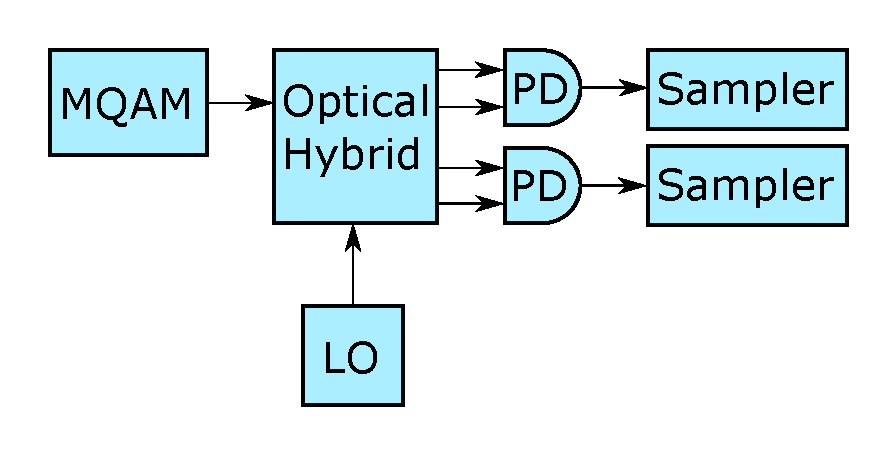
\includegraphics[width=\linewidth]{../img/scheme1.pdf}
\caption{Overview of the optical system being simulated.}
\label{fig:setup}
\end{figure}


\section{Required files}\label{Required files}

Header Files
\begin{table}[H]
\centering
\begin{tabulary}{1.0\textwidth}{|L|L|}
\hline
\textbf{File}              & \textbf{Description} 				            \\ \hline
netxpto.h                  & Generic purpose simulator definitions.	        \\ \hline
local\_oscillator.h        & Generates continuous coherent signal.            \\ \hline
balanced\_beam\_splitter.h & Mixes the two input signals into two outputs.    \\ \hline
homodyne\_reciever.h       & Performs coherent detection on the input signal. \\ \hline
sink.h                     & Closes any unused signals.                       \\ \hline
\end{tabulary}
\end{table}
%
Source Files
\begin{table}[H]
\centering
\begin{tabulary}{1.0\textwidth}{|L|L|}
\hline
\textbf{File}                & \textbf{Description} 					          \\ \hline
netxpto.cpp                  & Generic purpose simulator definitions.	          \\ \hline
local\_oscillator.cpp        & Generates continuous coherent signal.            \\ \hline
balanced\_beam\_splitter.cpp & Mixes the two input signals into two outputs.    \\ \hline
homodyne\_reciever.cpp       & Performs coherent detection on the input signal. \\ \hline
sink.cpp                     & Closes any unused signals.                       \\ \hline
\end{tabulary}
\end{table}


\section{System Input Parameters}

This system takes into account the following input parameters:
\begin{table}[H]
\centering
\begin{tabulary}{1.0\textwidth}{|C|C|}
\hline
\textbf{System Parameters} & \textbf{Description}                                                                   \\ \hline
numberOfBitsGenerated      & Gives the number of bits to be simulated                                               \\ \hline  
bitPeriod                  & Sets the time between adjacent bits                                                    \\ \hline 
samplesPerSymbol           & Establishes the number of samples each bit in the string is given                      \\ \hline
localOscillatorPower\_dBm1 & Sets the optical power, in units of dBm, of the varied amplitude signal                \\ \hline  
localOscillatorPower2      & Sets the optical power, in units of W, of the constant zero amplitude signal           \\ \hline  
localOscillatorPhase1      & Sets the initial phase of the local oscillator used for reference                      \\ \hline 
localOscillatorPhase2      & Sets the initial phase of the local oscillator used for signal                         \\ \hline  
transferMatrix             & Sets the transfer matrix of the beam splitter used in the homodyne detector            \\ \hline  
responsivity               & Sets the responsivity of the photodiodes used in the homodyne detector                 \\ \hline  
amplification              & Sets the amplification of the trans-impedance amplifier used in the homodyne detector  \\ \hline  
electricalNoiseAmplitude   & Sets the amplitude of the gaussian thermal noise added in the homodyne detector        \\ \hline
shotNoise                  & Chooses if quantum shot noise is used in the simulation                                \\ \hline
\end{tabulary}
\end{table}		

\section{Inputs}

This system takes no inputs.

\pagebreak
\section{Outputs}

The system outputs the following objects:
\begin{itemize}
\item Signals:
\begin{itemize}
\item Local Oscillator Optical Reference; (S$_{1}$)
\item Local Oscillator Optical Signal; (S$_{2}$)
\item Beam Splitter Outputs; (S$_{3}$, S$_{4}$)
\item Homodyne Detector Electrical Output; (S$_{5}$)
\end{itemize}
\end{itemize}	

\section{Simulation Results}\label{subsec:SHresults}

The following results show the dependence of the noise variance with the signal power, expressed in the value of the average photon number per pulse. Experimental results of the characterization of two different balanced homodyne detectors, obtained under the same conditions as the ones stipulated for the simulation, are presented in green and purple points alongside their respective quadratic fits. The thermal noise level is presented as a yellow line. The simulation results are presented as red points.

\begin{figure}[h]
\centering
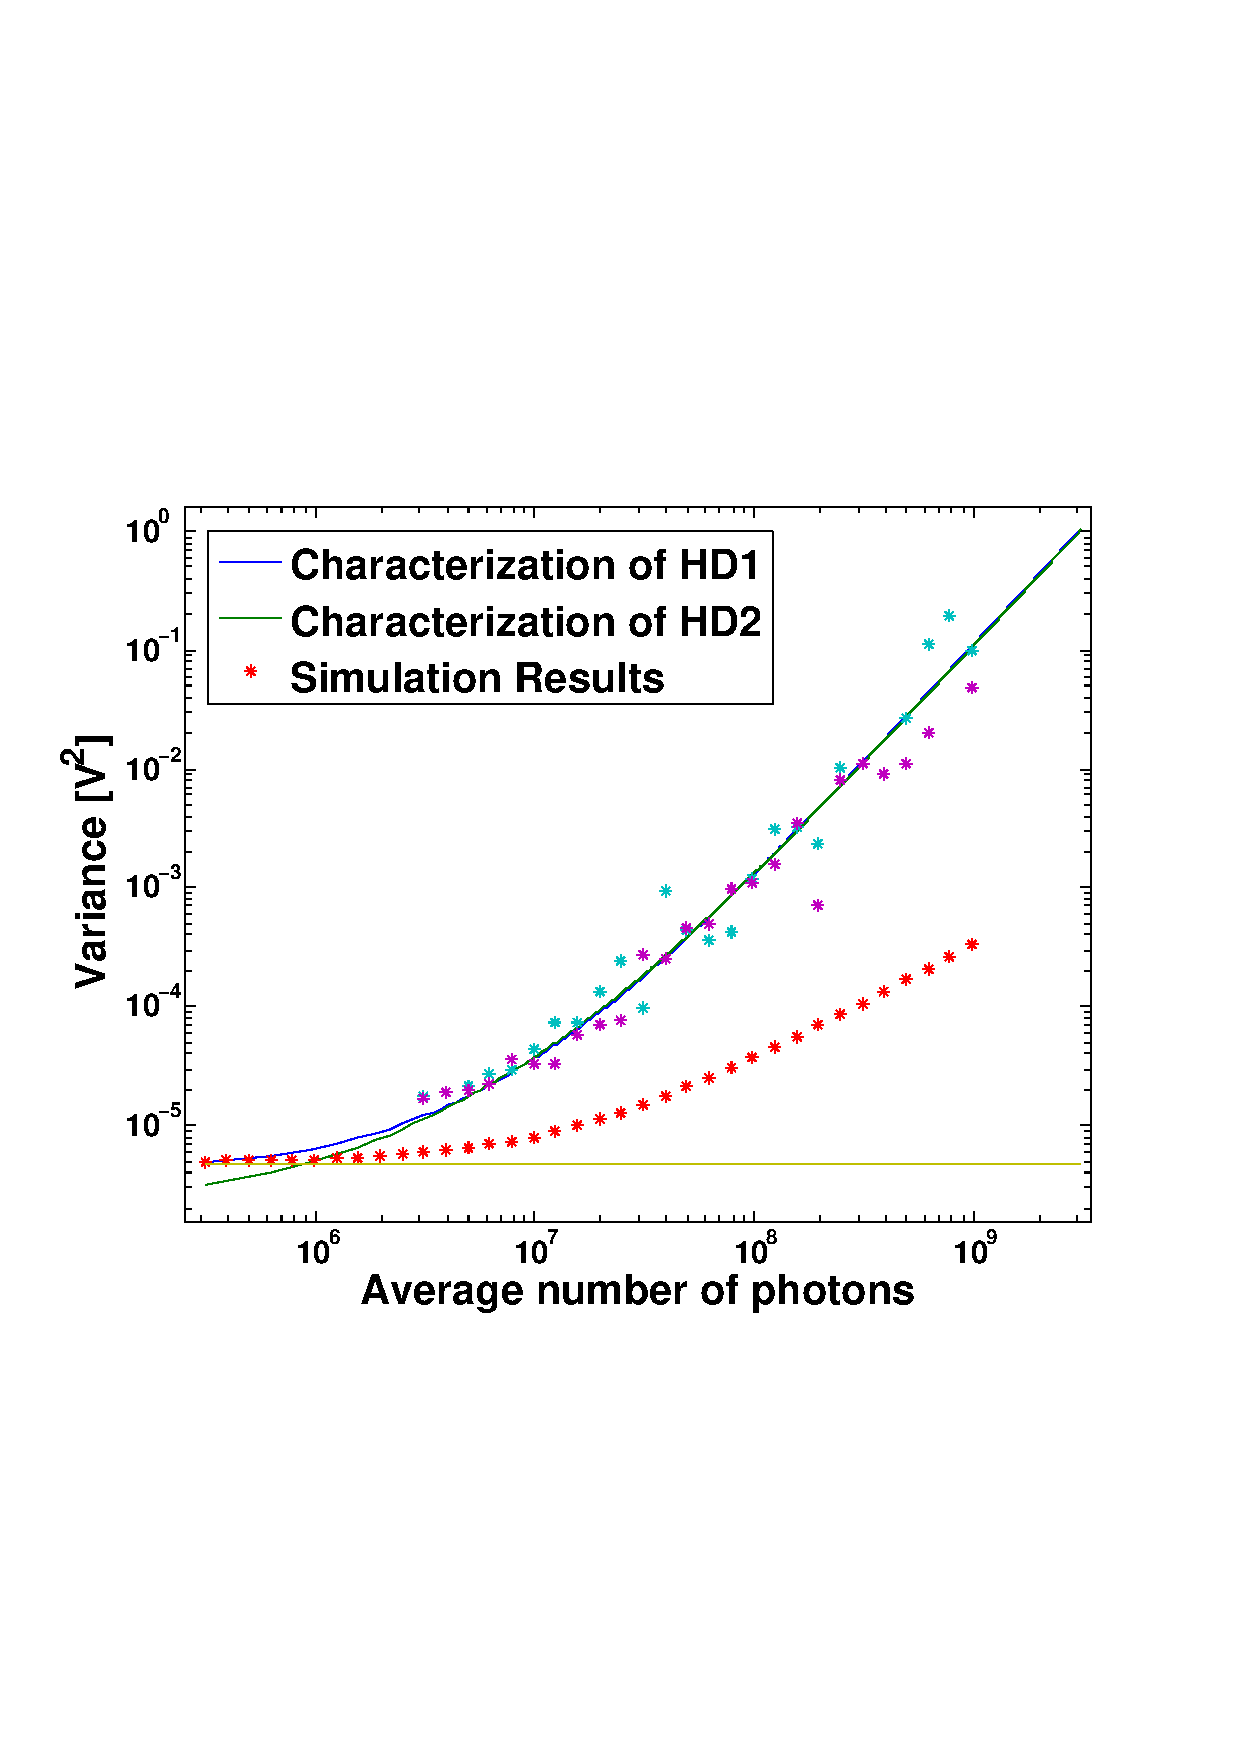
\includegraphics[width=\linewidth, trim= 0mm 60mm 0mm 70mm]{simulationresults1.pdf}
\caption{Noise variance in function of signal power.}
\label{fig:withquad}
\end{figure}

In Figure~\ref{fig:withquad} one can see that all results tend to the same value of thermal noise, however, simulated and experimental results evolve with different rates with signal power, this is mainly due to the existence of noise sources not considered in the simulation, moreover, setting the quadratic parameter in the experimental fit to 0 results yields the results presented in Figure~\ref{fig:withoutquad}, where the difference between the experimental fits and simulated results can be seen to not be as dramatic as before. The simulation and experimental  fits are, respectively:

\begin{table}[H]
\centering
\begin{tabular}{rc}
y=  & p$_0$+p$_1x$            \\
p$_0$= & 4.816$\times10^{-06}$\\
p$_1$= & 3.277$\times10^{-13}$ 
\end{tabular}
\end{table}

\begin{table}[H]
\centering
\begin{tabular}{rc}
y=  & p$_0$+p$_1x$+p$_2x^2$   \\
p$_0$= & 4.164$\times10^{-6}$ \\
p$_1$= & 2.183$\times10^{-12}$\\
p$_2$= & 1.069$\times10^{-19}$                 
\end{tabular}
\end{table}

\begin{table}[H]
\centering
\begin{tabular}{rc}
y=  & p$_0$+p$_1x$+p$_2x^2$   \\
p$_0$= & 2.357$\times10^{-6}$ \\
p$_1$= & 2.527$\times10^{-12}$\\
p$_2$= & 1.038$\times10^{-19}$                 
\end{tabular}
\end{table}

The linear parameters from the experimental fits are one order of magnitude above the linear parameter from the simulation fit, the reasons for this mismatch are still under study.

\begin{figure}[h]
\centering
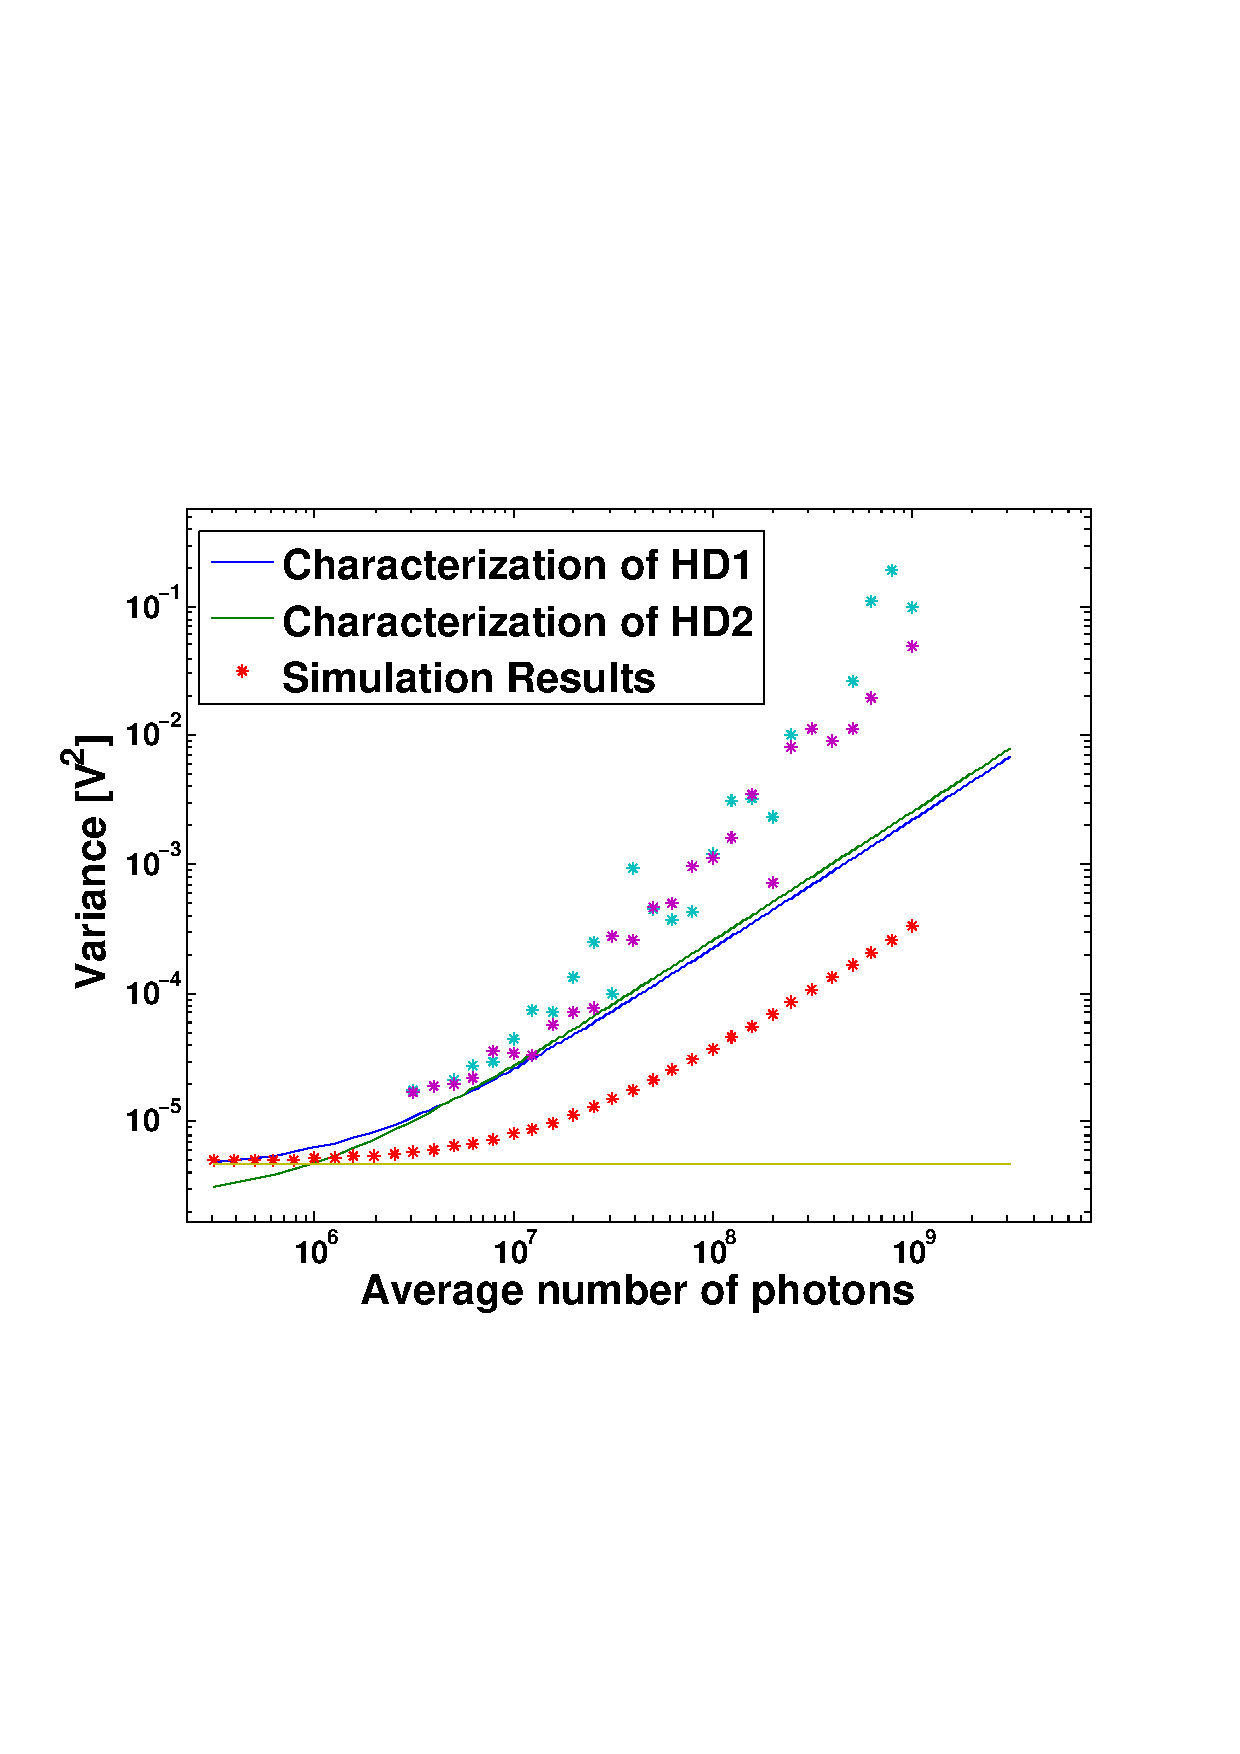
\includegraphics[width=\linewidth, trim= 0mm 60mm 0mm 70mm]{simulationresults2.pdf}
\caption{Noise variance in function of signal power with quadratic parameter deactivated.}
\label{fig:withoutquad}
\end{figure}

\section{Block Description}

\subsection{Homodyne Receiver}
\subfile{../../lib/tex/i_homodyne_reciever}

\subsection{Local Oscillator}
\subfile{../../lib/tex/localoscillator}

\subsection{Beam Splitter}
\subfile{../../lib/tex/beamsplitter}

\subsection{Photodiode}
\subfile{../../lib/tex/photodiode}

\subsection{Amplifier}
\subfile{../../lib/tex/ideal_amplifier}

\subsection{Electrical Filter}
\subfile{../../lib/tex/pulse_shaper}

\section{Known Problems}
\begin{enumerate}
    \item Homodyne Super-Block not functioning
\end{enumerate}


%\bibliographystyle{unsrt}
%\bibliography{bibliography}
\end{document} 
